%%%%%%%%%%%%%%%%%%%%%%%%%%%%%%%%%%%%%%%%%
% Beamer Presentation
% LaTeX Template
% Version 1.0 (10/11/12)
%
% This template has been downloaded from:
% http://www.LaTeXTemplates.com
%
% License:
% CC BY-NC-SA 3.0 (http://creativecommons.org/licenses/by-nc-sa/3.0/)
%
%%%%%%%%%%%%%%%%%%%%%%%%%%%%%%%%%%%%%%%%%

%----------------------------------------------------------------------------------------
%	PACKAGES AND THEMES
%----------------------------------------------------------------------------------------

\documentclass{beamer}

\mode<presentation> {
\usetheme{CambridgeUS}
%\usecolortheme{lily}

%\setbeamertemplate{footline} % To remove the footer line in all slides uncomment this line
%\setbeamertemplate{footline}[page number] % To replace the footer line in all slides with a simple slide count uncomment this line

\setbeamertemplate{navigation symbols}{} % To remove the navigation symbols from the bottom of all slides uncomment this line
}

\usepackage{graphicx} % Allows including images
\usepackage{booktabs} % Allows the use of \toprule, \midrule and \bottomrule in tables

\usepackage[utf8]{vietnam}

\setbeamerfont{footnote}{size=\tiny}

%----------------------------------------------------------------------------------------
%	TITLE PAGE
%----------------------------------------------------------------------------------------

\title[Khóa luận tốt nghiệp]{\textbf{Xây Dựng Ứng Dụng Trợ Lý Ảo Cho Máy Tính Sử Dụng Google Speech API}} % The short title appears at the bottom of every slide, the full title is only on the title page
\subtitle{Khóa luận tốt nghiệp Cử nhân Công nghệ thông tin}

\author{Bùi Trung Hải \and Phạm Ngọc Tuấn} % Your name
\institute[] % Your institution as it will appear on the bottom of every slide, may be shorthand to save space
{
GVHD: TS. Ngô Minh Nhựt \\
\medskip
Trường Đại học Khoa học tự nhiên TP. Hồ Chí Minh \\
Khoa Công nghệ thông tin \\
Hệ Cử nhân tài năng
}
\date{\today} % Date, can be changed to a custom date

\AtBeginSection[]{
    \begin{frame}
    \vfill
    \centering
    \begin{beamercolorbox}[sep=8pt,center,shadow=true,rounded=true]{title}
    \usebeamerfont{title}\insertsectionhead\par%
    \end{beamercolorbox}
    \vfill
    \end{frame}
}

\setbeamertemplate{caption}{\raggedright\insertcaption\par}
\graphicspath{{Figs/}}
\usepackage{multimedia}

\begin{document}

\begin{frame}
\titlepage % Print the title page as the first slide
\end{frame}

\begin{frame}
\frametitle{Nội dung} % Table of contents slide, comment this block out to remove it
\tableofcontents % Throughout your presentation, if you choose to use \section{} and \subsection{} commands, these will automatically be printed on this slide as an overview of your presentation
\end{frame}

%----------------------------------------------------------------------------------------
%	PRESENTATION SLIDES
%----------------------------------------------------------------------------------------

\section{Giới thiệu đề tài}

\subsection{Trợ lý ảo}

\begin{frame}
\frametitle{Trợ lý ảo là gì?}
\begin{itemize}
\item Ứng dụng trên máy tính hoặc thiết bị di động
\item Hỗ trợ người dùng thực hiện nhiều loại công việc
\item Nhận lệnh dưới dạng ngôn ngữ tự nhiên
\item Tăng tính hiệu quả và tạo ra sự tự nhiên trong giao tiếp giữa người và máy
\item Tạo cho người dùng những trải nghiệm mới và thú vị hơn khi sử dụng các thiết bị công nghệ
\end{itemize}
\end{frame}

\begin{frame}
\frametitle{Một số ứng dụng trợ lý ảo nổi tiếng}
\begin{columns}
\column{.33\textwidth}
\begin{minipage}[c][0.4\textheight][c]{\linewidth}
    \centering
    
\includegraphics[width=0.8\linewidth]{siri}
\end{minipage}
\begin{minipage}[c][0.4\textheight][c]{\linewidth}
    \centering
    
\includegraphics[width=0.8\linewidth]{googleass}
\end{minipage}
\column{.33\textwidth}
\begin{minipage}[c][0.4\textheight][c]{\linewidth}
    \centering
    
\includegraphics[width=0.8\linewidth]{cortana}
\end{minipage}
\begin{minipage}[c][0.4\textheight][c]{\linewidth}
    \centering
    
\includegraphics[width=0.8\linewidth]{bixby}
\end{minipage}
\column{.33\textwidth}
\begin{minipage}[c][0.4\textheight][c]{\linewidth}
    \centering
    
\includegraphics[width=0.8\linewidth]{alexa}
\end{minipage}
\begin{minipage}[c][0.4\textheight][c]{\linewidth}
    \centering
    
\includegraphics[width=0.8\linewidth]{facebookm}
\end{minipage}
\end{columns}
\end{frame}

\begin{frame}
\begin{figure}
\centering
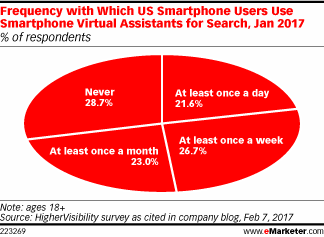
\includegraphics[scale=0.5]{emarketer_1}
\caption{Tần suất sử dụng trợ lý ảo của người dùng di động tại Mỹ\footnotemark}
\end{figure}

\footnotetext{\url{https://www.emarketer.com/Article/How-Do-People-Use-Virtual-Assistants-on-Their-Smartphones/1015251}}
\end{frame}

\begin{frame}
\begin{figure}
\centering
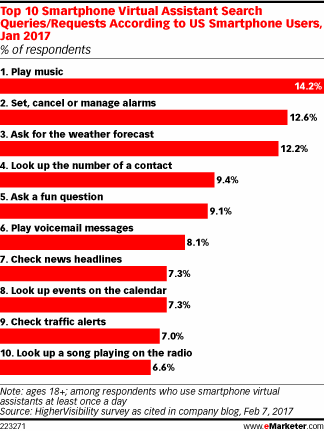
\includegraphics[scale=0.45]{emarketer_2}
\caption{Những chức năng được sử dụng nhiều nhất trên trợ lý ảo\footnotemark}
\end{figure}

\footnotetext{\url{https://www.emarketer.com/Article/How-Do-People-Use-Virtual-Assistants-on-Their-Smartphones/1015251}}
\end{frame}

\begin{frame}
\frametitle{Các vấn đề cần giải quyết}
\begin{itemize}
\item Phát hiện được keyword của người dùng để kích hoạt hệ thống
\item Nhận biết câu lệnh của người dùng với độ chính xác cao
\item Hiểu được câu lệnh của người dùng
\item Có được những phản hồi chính xác tương ứng với câu lệnh
\end{itemize}
\end{frame}

\subsection{Google Speech API}
\begin{frame}
\frametitle{Google Speech Recognition}
\begin{itemize}
\item Hệ thống nhận biết tiếng nói do Google nghiên cứu và phát triển
\item Được Google sử dụng trong Google Assistant, Google Home, Google Search,...
\item Độ chính xác đạt được hơn 95\%
\item Google cung cấp Google Speech API cho phép các nhà phát triển sử dụng Google Speech Recognition trong các ứng dụng.
\end{itemize}
\end{frame}

\subsection{Mục tiêu đề tài}

\begin{frame}
\frametitle{Mục tiêu đề tài}
\begin{itemize}
\item Tìm hiểu cấu trúc cơ bản của một ứng dụng trợ lý ảo
\item Xây dựng một ứng dụng trợ lý ảo trên máy tính, với các chức năng cơ bản:
    \begin{itemize}
    \item Hỏi đáp, tra cứu thông tin
    \item Hỏi giờ, thời tiết
    \item Phát nhạc
    \item Trò chuyện đơn giản
    \end{itemize}
\item Tìm hiểu và sử dụng những công cụ có sẵn để giải quyết các vấn đề và chức năng đã nêu.
\end{itemize}
\end{frame}

\section{Ứng dụng Alexa}

\subsection{Mô hình hoạt động}
\begin{frame}
\frametitle{Mô hình hoạt động}
\begin{figure}
\centering
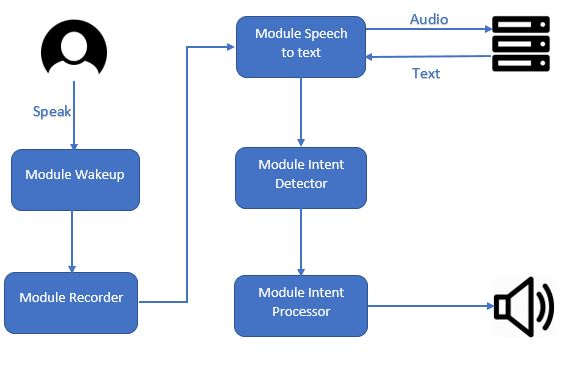
\includegraphics[scale=0.65]{system_flowchart}
\caption{Mô hình hoạt động của ứng dụng Alexa}
\end{figure}
\end{frame}

\subsection{Các module chính}
\begin{frame}
\frametitle{Các module chính}
\begin{itemize}
    \item \textbf{Microphone:} Thực hiện chức năng thu âm, sử dụng thư viện PyAudio.
    \item \textbf{WakeUp:} Thực hiện chức năng dò tìm keyword, sử dụng thư viện pocketsphinx.
    \item \textbf{Recorder:} Ghi âm lệnh của người dùng và nhận biết khi người dùng dừng nói để dừng ghi âm.
    \item \textbf{Speech to Text:} Dùng để chuyển dữ liệu tiếng nói thành văn bản, để đưa lệnh người dùng về văn bản và kiểm chứng lại keyword, sử dụng Google Speech to Text.
    \item \textbf{Text to Speech:} Chuyển đổi văn bản thành giọng nói để phản hồi lại người dùng, sử dụng iSpeech API.
    \item \textbf{Intent Detector:} Xác định ý nghĩa của mệnh lệnh người dùng, sử dụng thư viện Rasa NLU.
    \item \textbf{Intent Processor:} Xử lý và đưa ra kết quả cho mệnh lệnh của người dùng.
\end{itemize}
\end{frame}

\subsection{Các chức năng}
\begin{frame}
\frametitle{Các chức năng}
\begin{itemize}
    \item Thông báo giờ
    \item Thông báo thời tiết
    \item Phát nhạc
    \item Giao tiếp cơ bản
    \item Trả lời câu hỏi Wh-question
\end{itemize}
\end{frame}

\subsection{Giao diện ứng dụng}
\begin{frame}
\frametitle{Giao diện ứng dụng}
\begin{figure}
\centering
\href{Demo.mkv}{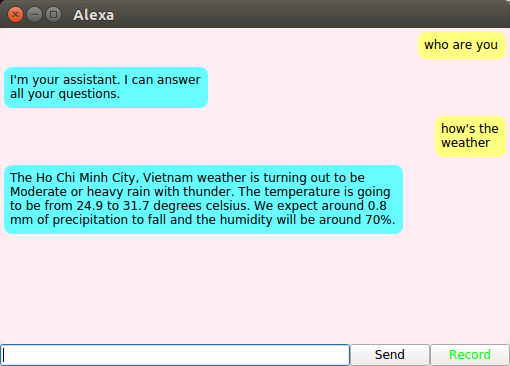
\includegraphics[scale=0.45]{interface}}
\caption{Giao diện của ứng dụng Alexa}
\end{figure}
\end{frame}

\section{Kết quả - Hướng phát triển}

\subsection{Kết quả}
\begin{frame}
\frametitle{Kết quả}
\begin{itemize}
\item Tìm hiểu được cấu trúc cơ bản của một ứng dụng trợ lý ảo.
\item Xây dựng được ứng dụng trợ lý ảo chạy trên nhiều nền tảng hệ điều hành khác nhau trên máy tính.
\item Ứng dụng có các chức năng cơ bản đáp ứng được mục tiêu đề ra.
\item Tìm hiểu được các thư viện xử lý âm thanh, speech to text, text to speech, natural language understanding,...
\item Áp dụng các kỹ thuật phát triển phần mềm và các webservice API.
\end{itemize}
\end{frame}

\subsection{Hạn chế}
\begin{frame}
\frametitle{Những điểm hạn chế}
\begin{itemize}
\item Ứng dụng chỉ hỗ trợ tiếng Anh.
\item Việc phản hồi không tạo thành một cuộc hội thoại mà chỉ dựa trên câu nói gần nhất của người dùng.
\item Số lượng chức năng ít.
\item Chức năng trả lời câu hỏi còn hạn chế.
\end{itemize}
\end{frame}

\subsection{Hướng phát triển}
\begin{frame}
\frametitle{Hướng phát triển}
\begin{itemize}
\item Hỗ trợ các ngôn ngữ khác tiếng Anh.
\item Cải thiện, làm cho việc giao tiếp trở nên tự nhiên hơn.
\item Tăng số lượng chức năng.
\item Cải thiện khả năng trả lời câu hỏi.
\item Thêm khả năng tương tác bằng hình ảnh.
\end{itemize}
\end{frame}

\section*{}

\begin{frame}
\huge{\centerline{Cảm ơn Thầy Cô và các bạn đã lắng nghe!}}
\end{frame}

\end{document} 
